\documentclass{amsart}
\usepackage{graphicx}
\graphicspath{{./}}
\usepackage{hyperref}
\usepackage{csvsimple}
\usepackage{longtable}
\usepackage{lscape}
\usepackage{epigraph}
\title{Proposals for R infrastructure for Fitting Categorical Ordered Variable Data Without MLE}
\author{Zulfikar Moinuddin Ahmed}
\date{\today}
\begin{document}
\maketitle

\section{Motivation}

For continuous variables, MLE fitting of Barndorff-Nielsen Generalised Hyperbolic Distribution has beautiful code in 'ghyp'.  I am interested in data from World Values Survey.  And Necessity, the Mother of Invention, shows up at my doorstep.  She says, "Ah, sonny boy, your Geometric Hyperbolic Distribution Shape looks a bit lifeless.  Don't you think it would be better that you interpolated the distribution and used least square fitting with GHD density directly?"
I replied, "Ah, Necessity, it's good to see you after such a long time.  Would you like to come in for some coffee?"

\section{Rough Outline}

I don't like to recode things that the R community has done well already in packages.  The world would be better if interpolation splines and such were not re-coded fifty million times.  And then there is a matter of least-square fitting of the densities directly rather than maximum likelihood on the data.  

But maximum likelihood estimation is theoretically justified more.  Well, no.  No law of Nature says that Generalised Hyperbolic distributions have to play any role at all for {\em Ordered Categorical Variables} and I can't show you her photograph here but Necessity, the Mother of Invention, is here with me and she seems to think it's okay not to use Maximum Likelihood Estimation.

\section{Log-Density Cubic Spline with Least Square fit of dghyp}

It is a democratic age and people are compelled by visually stunning displays in this age.  Nietzsche was wrong about how morality of people was invented and followed by herd mentality.  The idea appealed to him but here he was shallow.  He did not consider that it might simply be in our genetic inheritance of six million years.  His analysis was wrong there.  But he was right that in a democratic age people are compelled by glitz.  I will write about the deep error of Nietzsche's that extant values were concocted by individuals who gave their values to the people.  I used to believe him to some extent, until I realized that I would suffer deep envy of the hypothetical arbiters of the values of billions of people and didn't like that one bit.  For if everyone did follow someone's invented values, it should be mine.  Why should it be someone else's?  Fortunately Nature did it, and I never compete with Nature.  Some do, some do compete with Nature.  I revere and would not dream of competing with Nature.

\section{Code}

\begin{verbatim}
# GHD shape fitting

z<-cubicspline(1:4,CfGov[4,],xi=seq(0,5,by=0.001))
z<-z/(sum(z)*0.001)

fit_ghd_shape<-function( t, z ){
  delta <- t[2]-t[1]
  eps<-1e-6
  z<-z+eps
  z<-z/(sum(z)*delta)
  y<-log(z)
  objective<-function( theta ){
    yp <- log(dghyp( t, object=g(theta)))
    sum( (y-yp)^2*delta)
  }
  res<-optim( objective)
  res$solution
}
\end{verbatim}

\section{Intermediate Failure}

A slightly more detailed version of the code with a {\em failed} fit is next.

\begin{verbatim}
# GHD shape fitting

z<-cubicspline(1:4,CfGov[4,],xi=seq(0,5,by=0.01))
z<-z/(sum(z)*0.01)
t<-seq(0,5,by=0.01)
g<-function( theta ){
  lambda<-theta[1]
  mu <- theta[2]
  sigma <- theta[3]
  gamma <- theta[4]
  alpha.bar <- theta[5]
  out <- ghyp( lambda=lambda,mu=mu,sigma=sigma,
               gamma=gamma,alpha.bar=alpha.bar)
  out
}

fit_ghd_shape<-function( t, z0 ){
  delta <- t[2]-t[1]
  eps<-1e-6
  z<-cubicspline(1:length(z0),z0+eps,xi=t)
  z<-z/(sum(z)*delta)
  y<-log(abs(z)+eps)
  objective<-function( theta ){
    yp <- log(dghyp( t, object=g(theta))+eps)
    print(paste(length(y),length(yp)))
    out<-sum( (y-yp)^2*delta)
    if (is.na(out)){
      print(theta)
      print(yp)    
    }
    out
  }
  theta0 <-c( 0, 0.4, 1.2, 0.5, 0.11)
  lower0<-c(-1,-50,0,-100,0)
  upper0<-c(1,Inf,Inf,Inf,1)
  res<-optim( theta0, fn=objective,
              lower=lower0,
              upper=upper0,
              method="L-BFGS-B",control=list(trace=1))
  res$par
}
\end{verbatim}

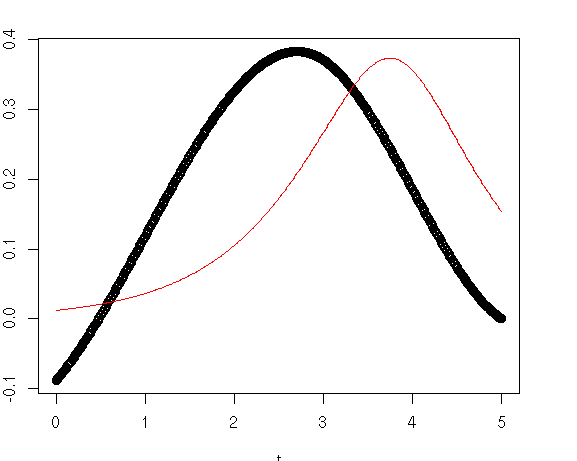
\includegraphics[scale=0.8]{intfail.png}

As you can see the fit failed.  But this is progress. I don't throw away the failures because that is how progress happens.  For people who are not experienced in science, it is very important to be quite unashamed and clear about the failures.  They are all valuable.  

\section{Justification of Slowing Down Here}

The fit is dreadful.  Some uninitiated minds would be driving immediately towards better looking fits.  I would often myself.  But I have experience with Mittag-Leffler functions and other special functions from R. Mainardi and others working in fractional heat equation and other exotic special functions; I have seen the complexity of the zeta and other special functions in mathematics.  And the form of Generalised Hyperbolic Distribution density is similar to those with various Bessel functions of the second kind and so on, and I am extremely hesitant to rush headlong into trying to brute force my way to fitting in this case.  The bad fit is a minor inconvenience.  I stopped before {\em substantial problem s arise} in this case which is that I am totally lost about the sensitivity of $g(\theta)$ to the parameters in shape and spend six months of frustrations trying to find parameters and initial values blindly.  Therefore the stopping point above is efficient.

\section{The Messy Manual Checks}

Just in case you think that Zulf has the perfect divine intuition that leads to a straightforward victory, I have some news for you.

This is what my manual tests look like.

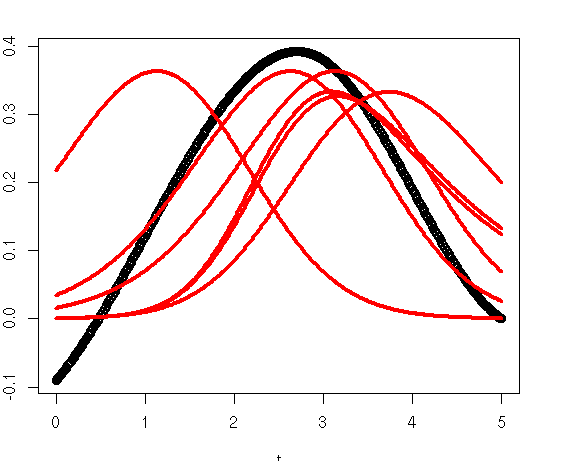
\includegraphics[scale=0.8]{manual_tests.png}

Manual tests exist to understand the 
model a bit better.

\section{A New Sign of Hope}

Around 9:44 pm, Zulf finds a reasonable hope, a slightly better fit to the curve.

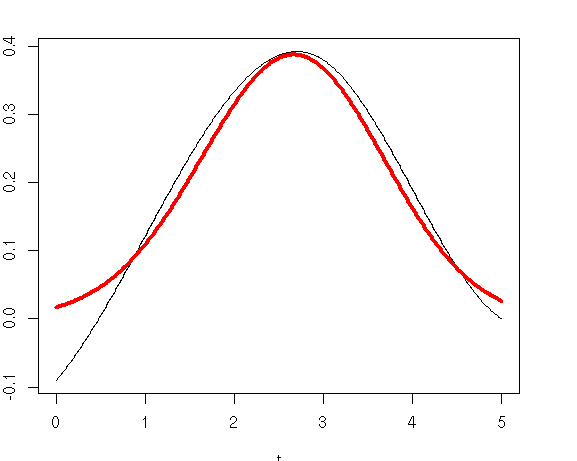
\includegraphics[scale=0.8]{betterfit_may15_2021.png}

This is looking quite nice for this example but other cases could be beset with difficulties.

\section{Another Example}

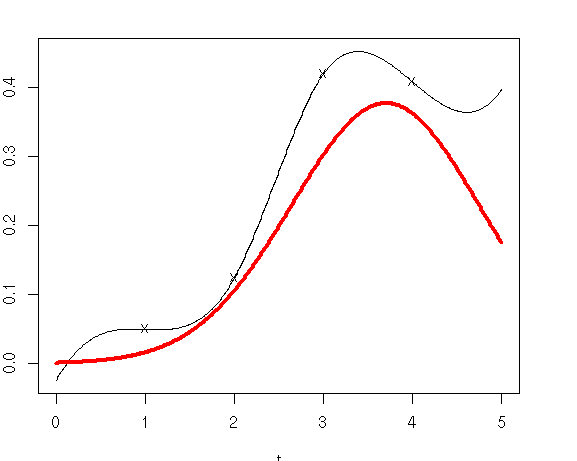
\includegraphics[scale=0.8]{fit2_cfgivt2.png}

This is quite delicate amd the fit could improve.

\section{Slight tweaks to Fitting}

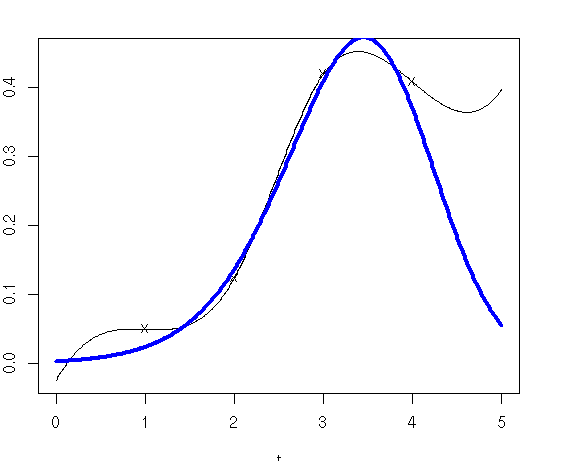
\includegraphics[scale=0.8]{fit3_cfgovt2.png}


\section{More fudging}

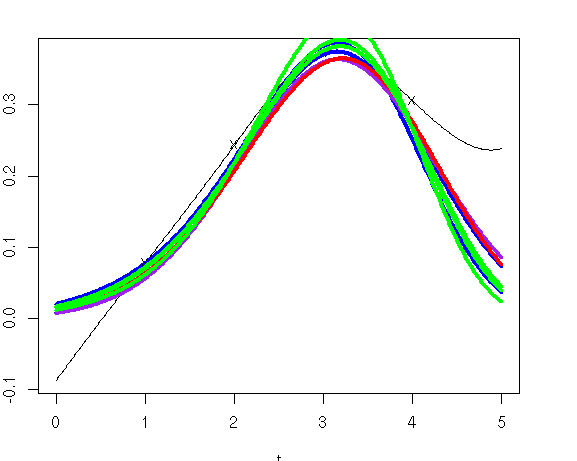
\includegraphics[scale=0.8]{fit2_cfgovt5.png}


\section{State of Code}

\begin{verbatim}
# GHD shape fitting

z<-cubicspline(1:4,CfGov[4,],xi=seq(0,5,by=0.01))
z<-z/(sum(z)*0.01)
t<-seq(0,5,by=0.01)
g<-function( theta ){
  lambda<-theta[1]
  mu <- theta[2]
  sigma <- theta[3]
  gamma <- theta[4]
  alpha.bar <- theta[5]
  out <- ghyp( lambda=lambda,mu=mu,sigma=sigma,
               gamma=gamma,alpha.bar=alpha.bar)
  out
}

fit_ghd_shape<-function( t, z0 ){
  delta <- t[2]-t[1]
  eps<-1e-6
  z<-cubicspline(1:length(z0),z0,xi=t)
  z[z<eps]<-eps
  z<-z/(sum(z[t>0.5 & t<4.5])*delta)
  y<-z
  objective<-function( theta ){
    yp <- dghyp( t, object=g(theta))
    out<-sum( delta*(y[t>0.9 & t<4.3]- yp[t>0.9 & t < 4.3])^2)
    if (is.na(out)){
      print(theta)
      print(yp)    
    }
    out
  }
  theta0 <-c(-3.0,3.5,1.1,0.0,1.0)
  lower0<-c(-Inf,0,0.001,-Inf,0)
  upper0<-c(Inf,100,Inf,Inf,Inf)
  res<-optim( theta0, fn=objective,
              lower=lower0,
              upper=upper0,
              method="L-BFGS-B",control=list(trace=1,maxit=5000))
  res$par
}
\end{verbatim}

\section{Another Fit}

\begin{verbatim}
plot(t,z,type='l')
lines( t,
dghyp(t,object=g(theta)),col='green',lwd=4)
points(1:4,CfGov[6,],pch='x')
\end{verbatim}

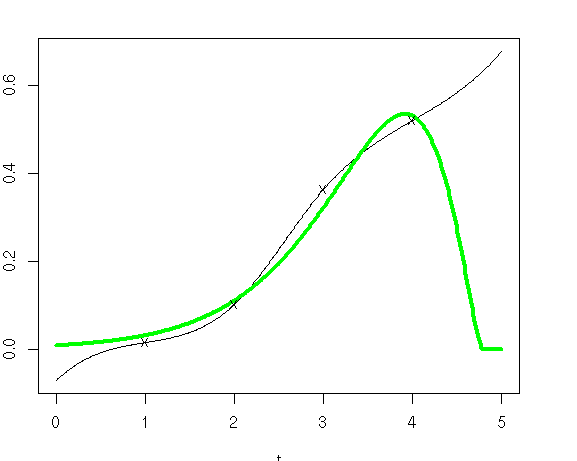
\includegraphics[scale=0.8]{fit_cfgovt6.png}

\end{document}